\section{Geom\-PQP2DPoint  Class Reference}
\label{class_GeomPQP2DPoint}\index{GeomPQP2DPoint@{Geom\-PQP2DPoint}}
2D point robot. 


{\tt \#include $<$geom\-PQP.h$>$}

Inheritance diagram for Geom\-PQP2DPoint:\begin{figure}[H]
\begin{center}
\leavevmode
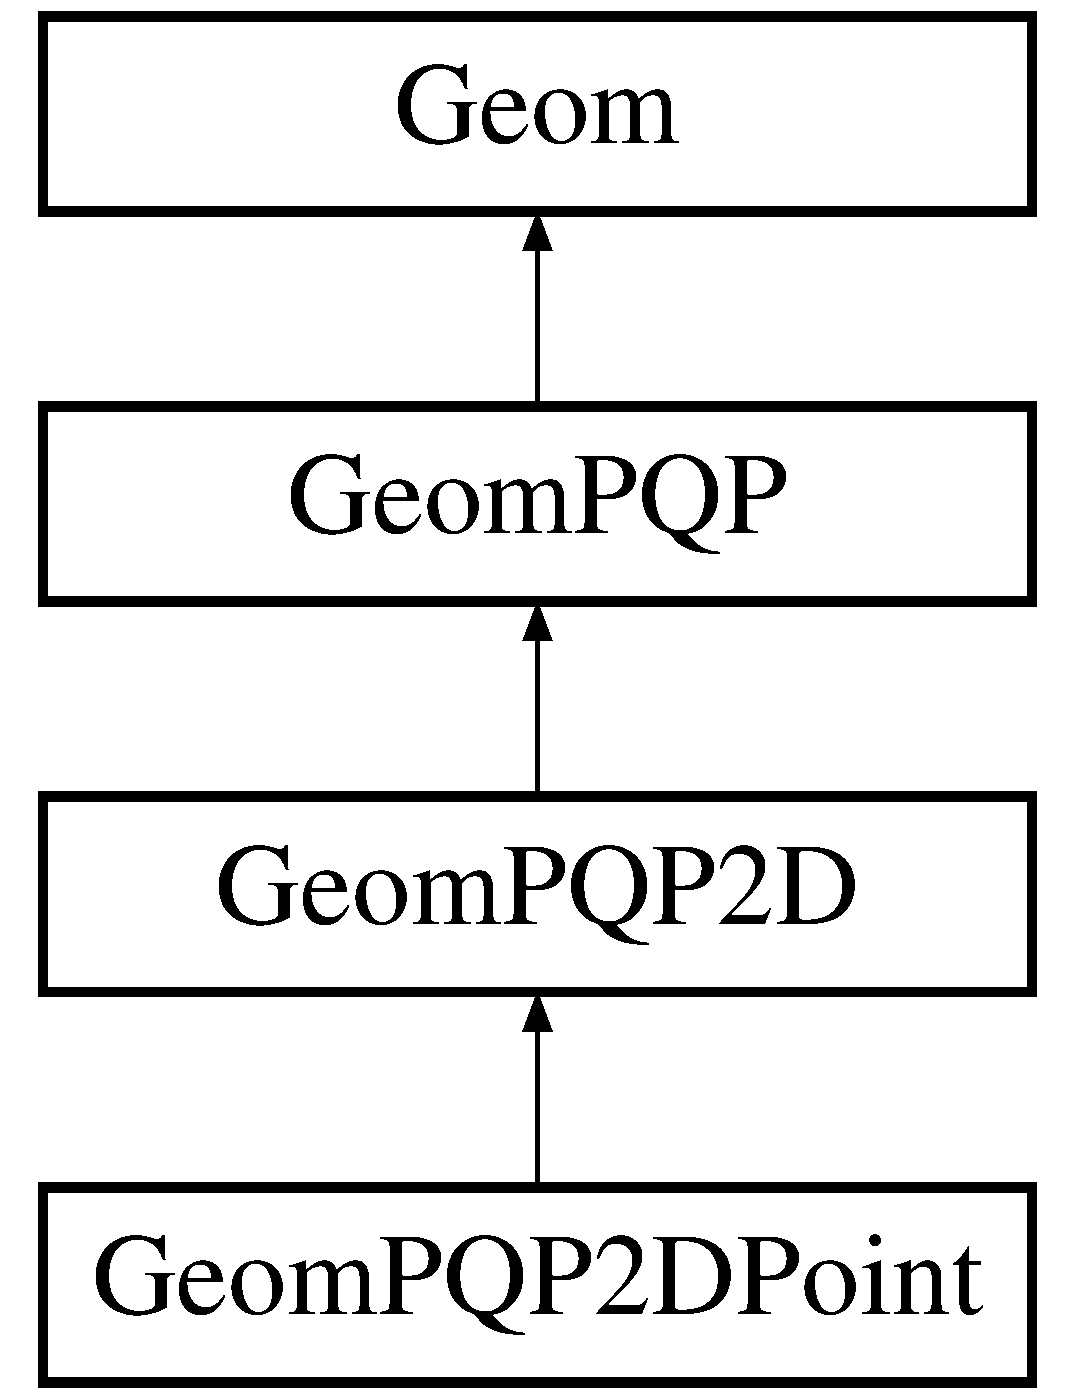
\includegraphics[height=4cm]{class_GeomPQP2DPoint}
\end{center}
\end{figure}
\subsection*{Public Methods}
\begin{CompactItemize}
\item 
{\bf Geom\-PQP2DPoint} (string path)
\item 
virtual {\bf $\sim$Geom\-PQP2DPoint} ()
\item 
virtual bool {\bf Collision\-Free} (const {\bf MSLVector} \&q)
\begin{CompactList}\small\item\em Return true if the robot(s) and obstacles are not in collision.\item\end{CompactList}\item 
virtual double {\bf Distance\-Comp} (const {\bf MSLVector} \&q)
\begin{CompactList}\small\item\em Compute the distance of the closest point on the robot to the obstacle region.\item\end{CompactList}\end{CompactItemize}


\subsection{Detailed Description}
2D point robot.





\subsection{Constructor \& Destructor Documentation}
\index{GeomPQP2DPoint@{Geom\-PQP2DPoint}!GeomPQP2DPoint@{GeomPQP2DPoint}}
\index{GeomPQP2DPoint@{GeomPQP2DPoint}!GeomPQP2DPoint@{Geom\-PQP2DPoint}}
\subsubsection{\setlength{\rightskip}{0pt plus 5cm}Geom\-PQP2DPoint::Geom\-PQP2DPoint (string {\em path} = "")}\label{class_GeomPQP2DPoint_a0}


\index{GeomPQP2DPoint@{Geom\-PQP2DPoint}!~GeomPQP2DPoint@{$\sim$GeomPQP2DPoint}}
\index{~GeomPQP2DPoint@{$\sim$GeomPQP2DPoint}!GeomPQP2DPoint@{Geom\-PQP2DPoint}}
\subsubsection{\setlength{\rightskip}{0pt plus 5cm}Geom\-PQP2DPoint::$\sim$Geom\-PQP2DPoint ()\hspace{0.3cm}{\tt  [inline, virtual]}}\label{class_GeomPQP2DPoint_a1}




\subsection{Member Function Documentation}
\index{GeomPQP2DPoint@{Geom\-PQP2DPoint}!CollisionFree@{CollisionFree}}
\index{CollisionFree@{CollisionFree}!GeomPQP2DPoint@{Geom\-PQP2DPoint}}
\subsubsection{\setlength{\rightskip}{0pt plus 5cm}bool Geom\-PQP2DPoint::Collision\-Free (const {\bf MSLVector} \& {\em q})\hspace{0.3cm}{\tt  [virtual]}}\label{class_GeomPQP2DPoint_a2}


Return true if the robot(s) and obstacles are not in collision.



Reimplemented from {\bf Geom\-PQP} {\rm (p.\,\pageref{GeomPQP_a4})}.\index{GeomPQP2DPoint@{Geom\-PQP2DPoint}!DistanceComp@{DistanceComp}}
\index{DistanceComp@{DistanceComp}!GeomPQP2DPoint@{Geom\-PQP2DPoint}}
\subsubsection{\setlength{\rightskip}{0pt plus 5cm}double Geom\-PQP2DPoint::Distance\-Comp (const {\bf MSLVector} \& {\em q})\hspace{0.3cm}{\tt  [virtual]}}\label{class_GeomPQP2DPoint_a3}


Compute the distance of the closest point on the robot to the obstacle region.



Reimplemented from {\bf Geom\-PQP} {\rm (p.\,\pageref{GeomPQP_a5})}.

The documentation for this class was generated from the following files:\begin{CompactItemize}
\item 
{\bf geom\-PQP.h}\item 
{\bf geom\-PQP.C}\end{CompactItemize}
